\section{Community-Level Results}
\label{sec:community-level-results}

Figure~\ref{fig:community_ate} shows the community-level ATE estimates across the five annotation paradigms for communities with at least one significant effect. The complete ATE table for all nine communities passing the minimum threshold requirement of 50 articles is provided in Appendix~\ref{sec:appendix-community-ate}.

\begin{figure}[h!]
    \centering
    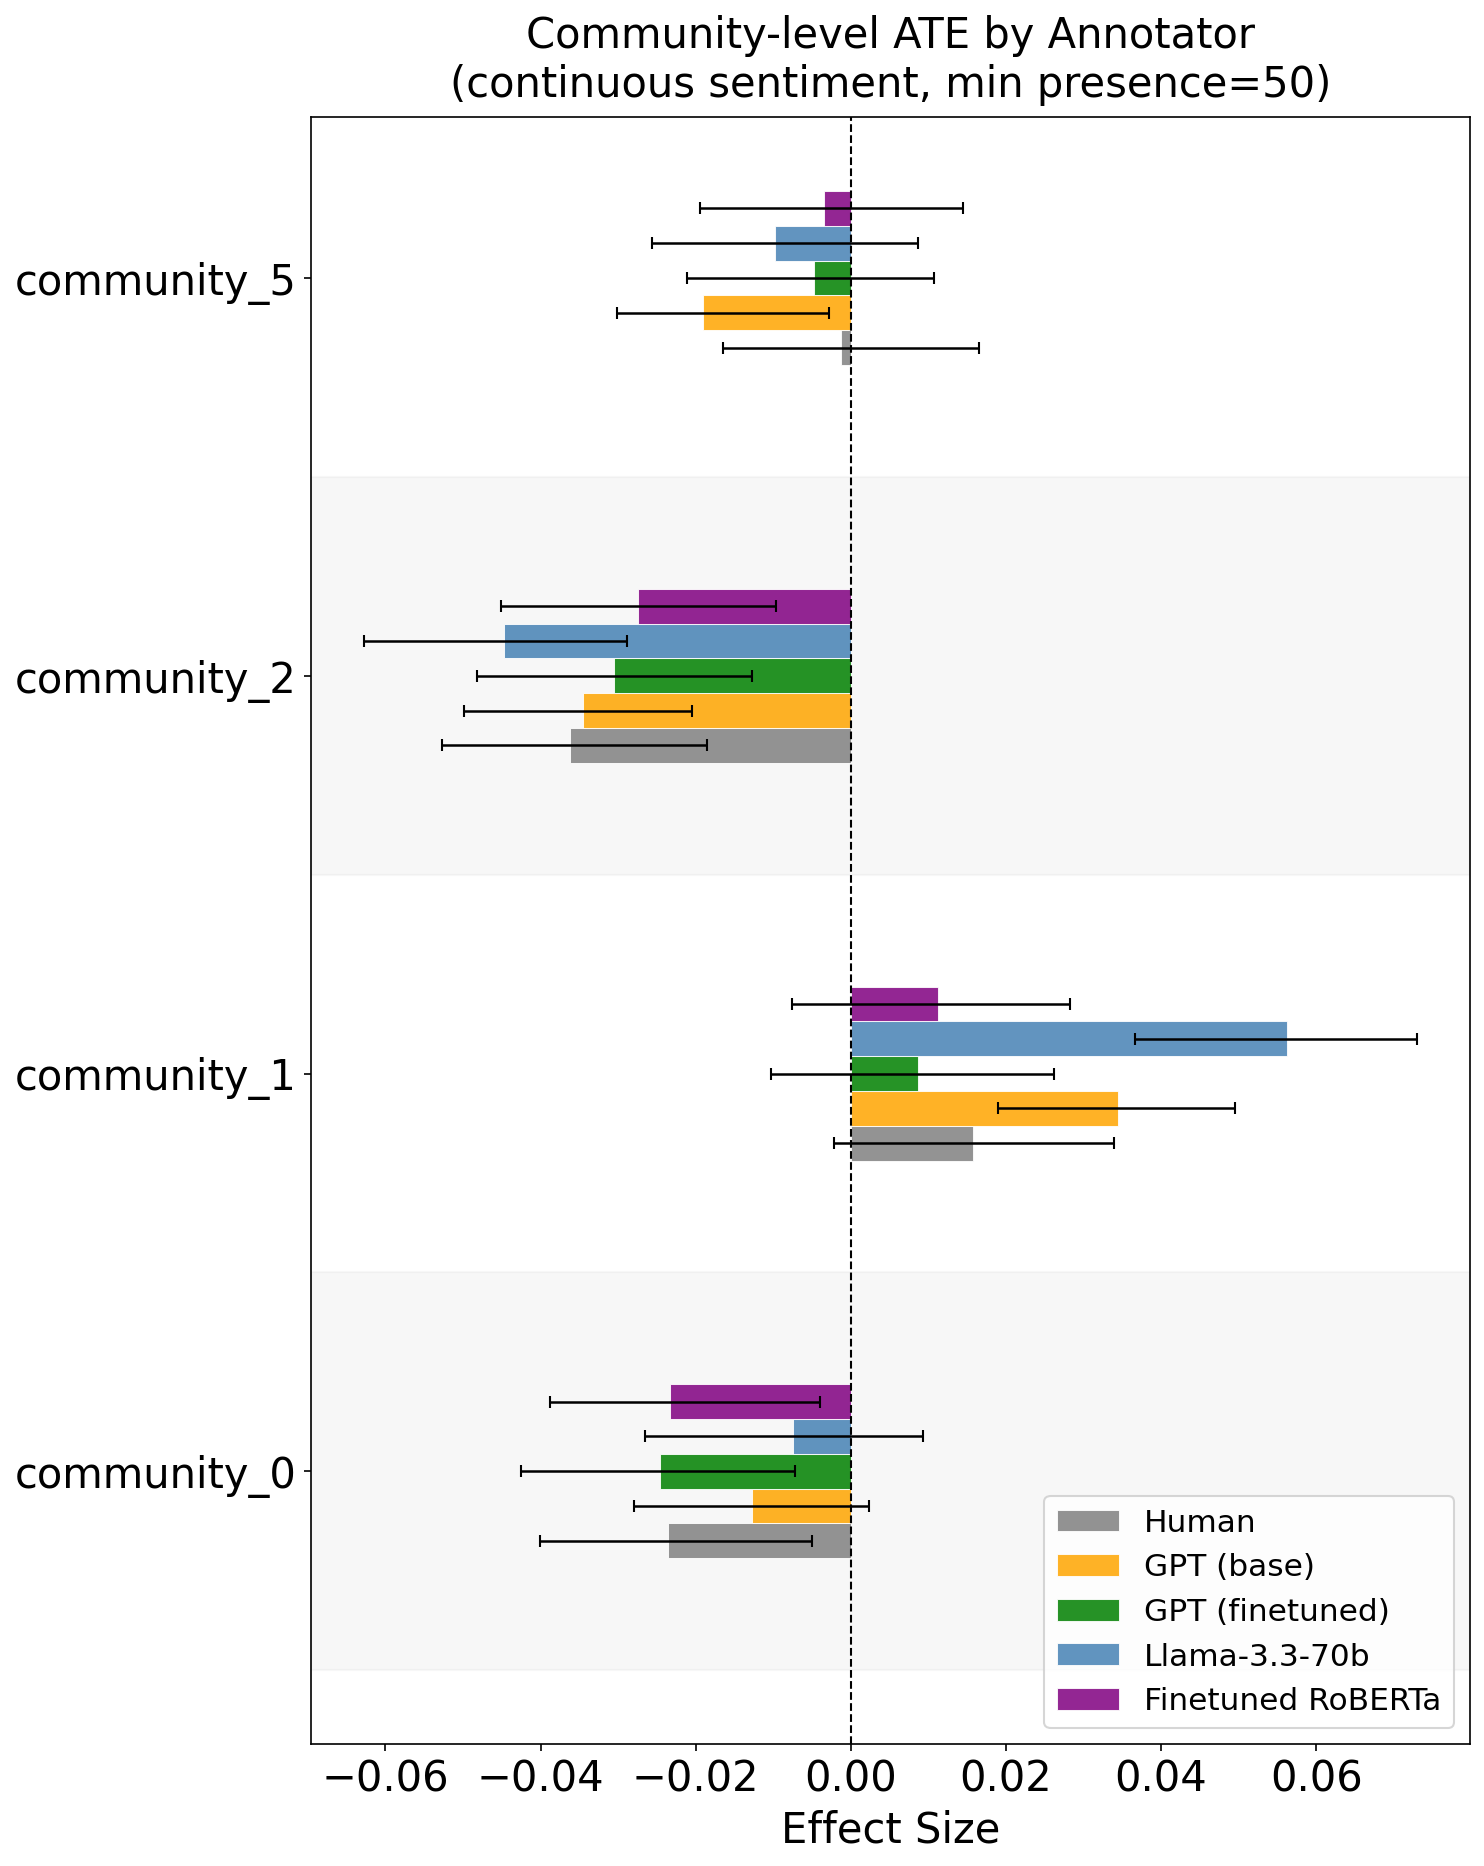
\includegraphics[width=0.7\textwidth]{sections/images/causal_analysis/media_split/ate_communities.png}
    \caption{Community-level ATE (continuous sentiment) for communities with significant effects in any annotation paradigm.}
    \label{fig:community_ate}
\end{figure}

Throughout this chapter, the ideology label is encoded on a $[0, 2]$ scale where $0 = $ Left, $1 = $ Center, and $2 = $ Right. A \emph{negative} ATE therefore means that increasing positive sentiment toward the treatment topic shifts the predicted ideology label \emph{toward Left} (i.e.\ down the scale), while a \emph{positive} ATE shifts it toward Right (up the scale).

Four of nine qualifying communities produce at least one significant ATE, yielding 14 significant cells across the five paradigms. Community~2 (Public Health) achieves full cross-paradigm replication (5/5 significant), a first at the community level.

\subsubsection{Community~2: Public Health}

Community~2 is the headline community-level finding. All five paradigms produce significant negative ATEs: Human $-0.036$, Fine-tuned RoBERTa $-0.027$, baseline GPT $-0.035$, Fine-tuned GPT $-0.031$ and Llama $-0.045$. Improving sentiment toward public health topics shifts ideology predictions leftward, consistent with public health being a liberal-coded policy area in the US political landscape. This community includes three of the top~20 topics from Table~\ref{tab:multi-continuous-full}: Coronavirus ($N = 441$), Healthcare ($N = 373$), and Public Health ($N = 297$). Of these topics, healthcare has the strongest individual signal, showing a significant leftward shift across all paradigms. The coronavirus and public health topics generally show leftward ATEs (baseline GPT and Llama being exceptions in the public health case), but neither topic reaches significance individually. The community-level aggregation preserves both direction and significance.

\subsubsection{Community~0: White House and Congress}

Three of five paradigms reach significance in Community~0, all in the negative direction: Human $-0.024$, Fine-tuned RoBERTa $-0.023$, and Fine-tuned GPT $-0.025$. Baseline GPT ($-0.013$) and Llama ($-0.008$) agree directionally but do not reach significance. Fine-tuning has a notable effect on the GPT family in this community: the baseline GPT estimate is non-significant at $-0.013$, while Fine-tuned GPT reaches significance at $-0.025$, moving the effect size closer to the human estimate of $-0.024$. This community includes Politics ($N = 1{,}520$), White House ($N = 701$), and Barack Obama ($N = 286$, significant across all five paradigms) from the top~20 topics. The negative direction is consistent with the topic-level finding that Barack Obama sentiment shifts ideology predictions leftward: the community-level effect aggregates this partisan signal with the broadly distributed but individually non-significant Politics and White House topics.

\subsubsection{Community~1: Elections and Campaigns}

Community~1 exhibits significant effects only under the two zero-shot paradigms: baseline GPT $+0.034$ and Llama $+0.056$. Human ($+0.016$), Fine-tuned RoBERTa ($+0.011$), and Fine-tuned GPT ($+0.009$) estimate positive effects that do not reach significance. This is the largest community by article count ($N = 3{,}628$) and contains the most top~20 topics: Elections ($N = 1{,}709$), Donald Trump ($N = 1{,}424$), Presidential Elections ($N = 1{,}331$), Republican Party ($N = 293$), Joe Biden ($N = 288$), Hillary Clinton ($N = 279$), and Democratic Party ($N = 261$). Despite containing topics with large individual ATEs in both directions (Donald Trump and Republican Party positive; Joe Biden, Hillary Clinton, and Democratic Party negative), the community-level effect is positive, suggesting that the rightward signals dominate when sentiments are aggregated. The fact that only zero-shot paradigms detect a significant aggregate effect, while human annotations do not, raises the possibility that the zero-shot models are responding to surface-level cues rather than genuine ideological structure. We return to this point in Section~\ref{sec:shortcut-learning}.

\subsubsection{Community~5: Environment and Fiscal Policy}

Only baseline GPT produces a significant effect in Community~5: $-0.019$. All other paradigms estimate small negative effects (Human $-0.001$, Fine-tuned RoBERTa $-0.003$, Fine-tuned GPT $-0.005$, Llama $-0.010$) with confidence intervals spanning zero. The community includes Economy and Jobs ($N = 462$) from the top~20 topics. Baseline GPT appears more sensitive to the sentiment-ideology relationship in this policy domain than other paradigms, though the effect does not replicate.

\subsubsection{Cross-Paradigm Alignment}

Among the significant communities, the fine-tuned models show the closest alignment with human annotations. In Community~0, Fine-tuned GPT ($-0.025$) and Fine-tuned RoBERTa ($-0.023$) bracket the human estimate ($-0.024$), with deviations of $0.001$ and $0.001$ respectively. In Community~2, Fine-tuned GPT ($-0.031$) is the closest paradigm to Human ($-0.036$) with a deviation of $0.005$, followed by baseline GPT ($-0.035$, deviation $0.001$) and Fine-tuned RoBERTa ($-0.027$, deviation $0.009$). Llama-3.3-70B produces the largest magnitudes in Community~2 ($-0.045$) and Community~1 ($+0.056$), consistent with its tendency toward inflated effect sizes at the topic level.

\subsection{Community-Level Mediation Analysis}
\label{sec:community-mediation-results}

We next decompose the community-level effects into direct and indirect components using natural effect mediation. Communities 0 (White House and Congress), 1 (Elections and Campaigns), and 2 (Public Health) were selected because all or nearly all paradigms produced significant ATEs for them in Section~\ref{sec:community-level-results}, making them the natural candidates for a mediation follow-up. We examine two complementary pathway configurations: (a) Community~1 as treatment with Communities~0 and~2 serving in turn as mediators ($1 \to 0$ and $1 \to 2$), and (b) the contrast direction, with Communities~0 and~2 as treatments and Community~1 as the mediator ($0 \to 1$ and $2 \to 1$). Table~\ref{tab:community-mediation-summary} summarizes the three communities and their article counts; full numerical tables appear in Appendix~\ref{sec:appendix-community-mediation}.

\begin{table}[h]
  \centering
  \begin{tabular}{clr}
    \toprule
    \textbf{Community} & \textbf{Name} & \textbf{Articles} \\
    \midrule
    0 & White House and Congress & 2,743 \\
    1 & Elections and Campaigns  & 3,628 \\
    2 & Public Health            & 1,116 \\
    \bottomrule
  \end{tabular}
  \caption{Communities retained for mediation analysis and their article counts.}
  \label{tab:community-mediation-summary}
\end{table}

Figures~\ref{fig:mediation_community_1_treatment} and~\ref{fig:mediation_community_1_mediator} show the decomposition of Total Effect (TE) into Natural Direct Effect (NDE) and Natural Indirect Effect (NIE) for the four pathways across all five paradigms.

\begin{figure}[h]
    \centering
    \begin{subfigure}[b]{0.48\textwidth}
        \centering
        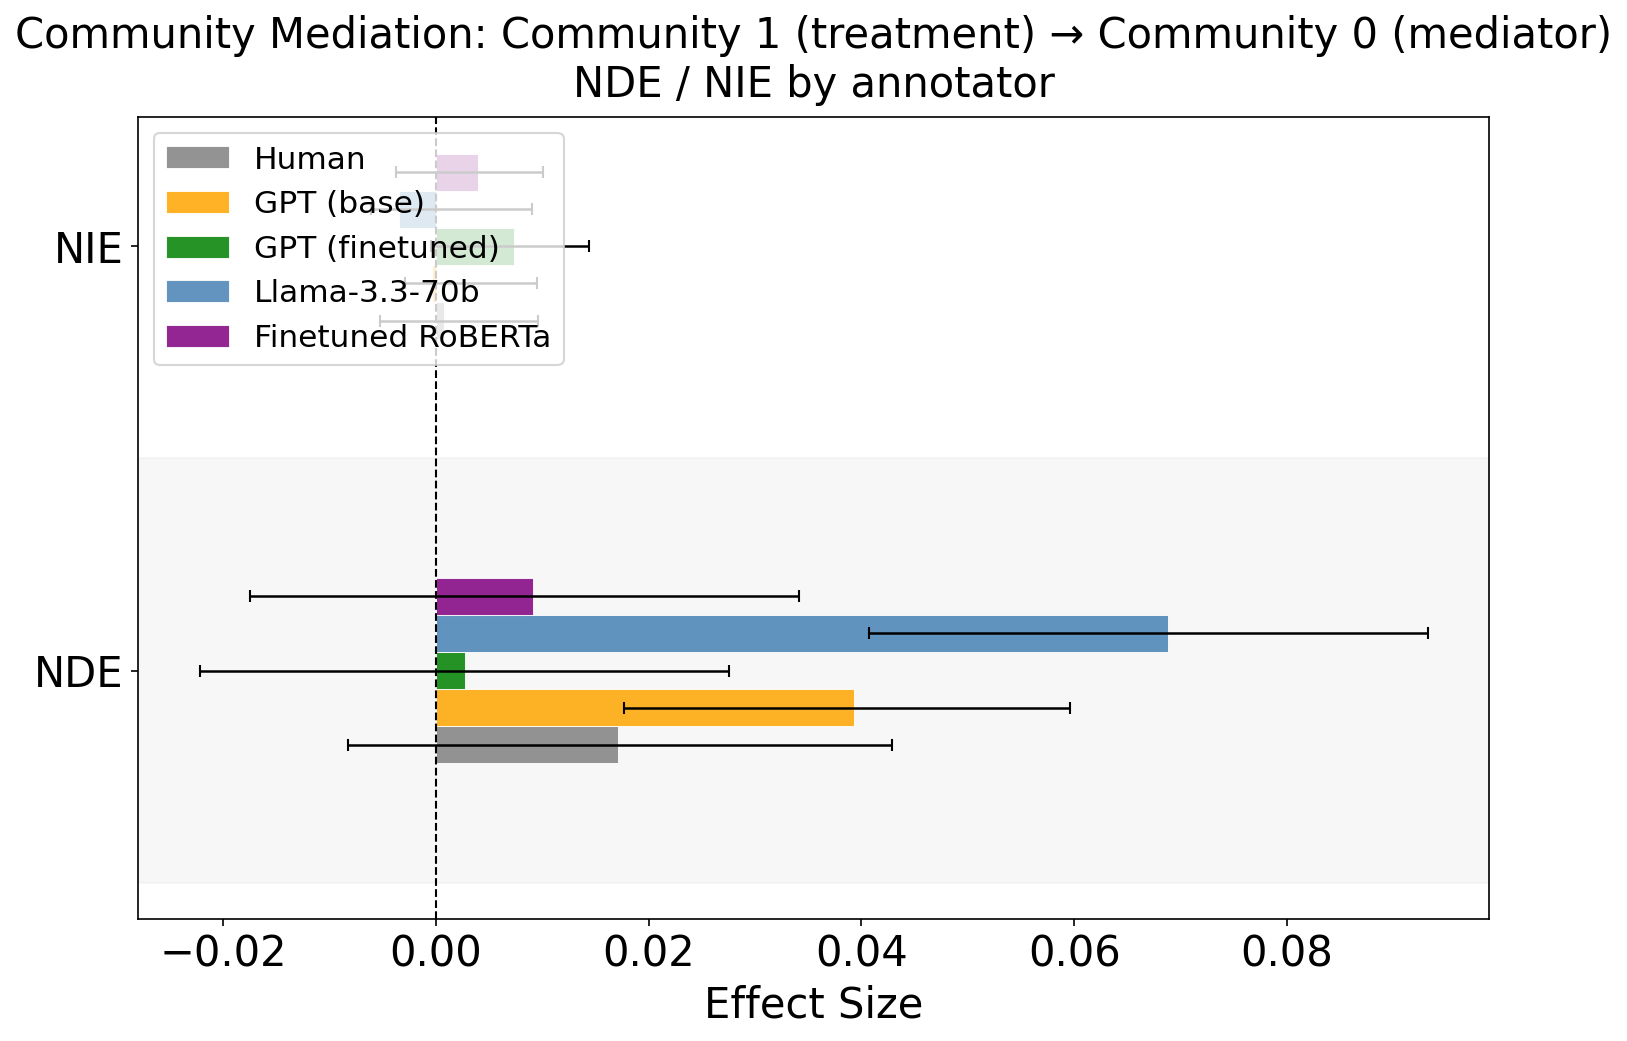
\includegraphics[width=\textwidth]{sections/images/causal_analysis/media_split/mediation_community_1_0.png}
        \caption{$1 \to 0$}
        \label{fig:mediation_1_0}
    \end{subfigure}
    \hfill
    \begin{subfigure}[b]{0.48\textwidth}
        \centering
        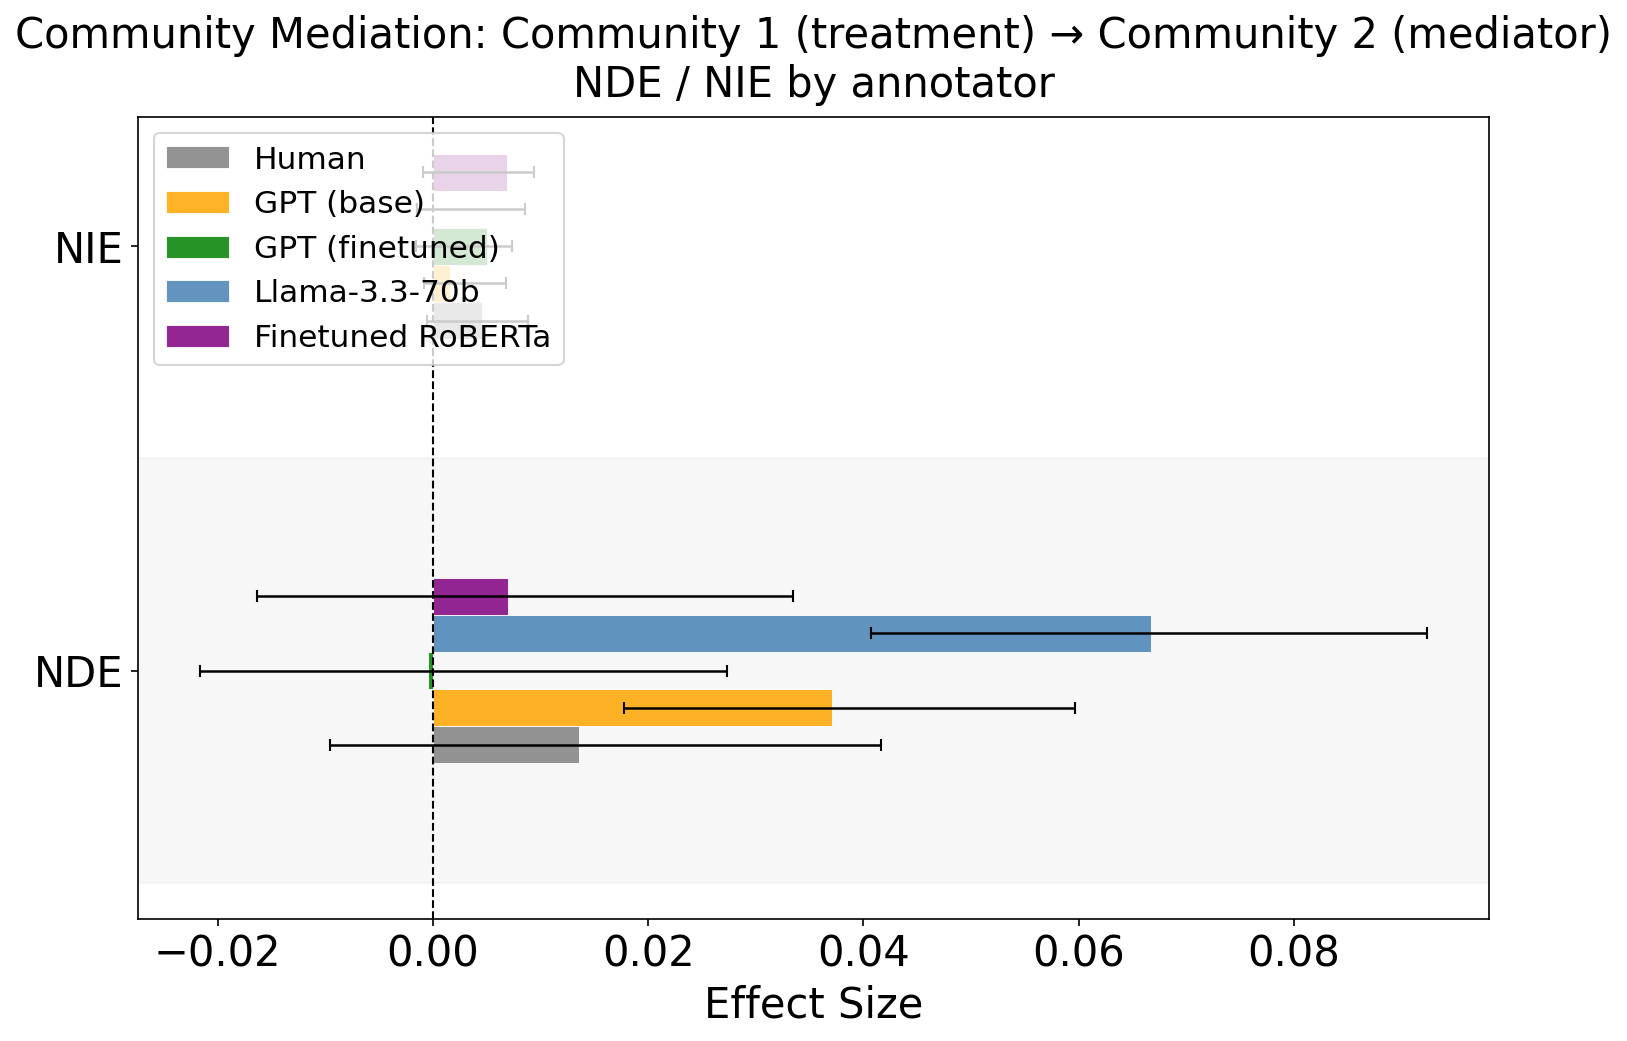
\includegraphics[width=\textwidth]{sections/images/causal_analysis/media_split/mediation_community_1_2.png}
        \caption{$1 \to 2$}
        \label{fig:mediation_1_2}
    \end{subfigure}
    \caption{Mediation decomposition with Community~1 (Elections and Campaigns) as treatment and Communities~0 (White House and Congress) and~2 (Public Health) as mediators.}
    \label{fig:mediation_community_1_treatment}
\end{figure}

\begin{figure}[h]
    \centering
    \begin{subfigure}[b]{0.48\textwidth}
        \centering
        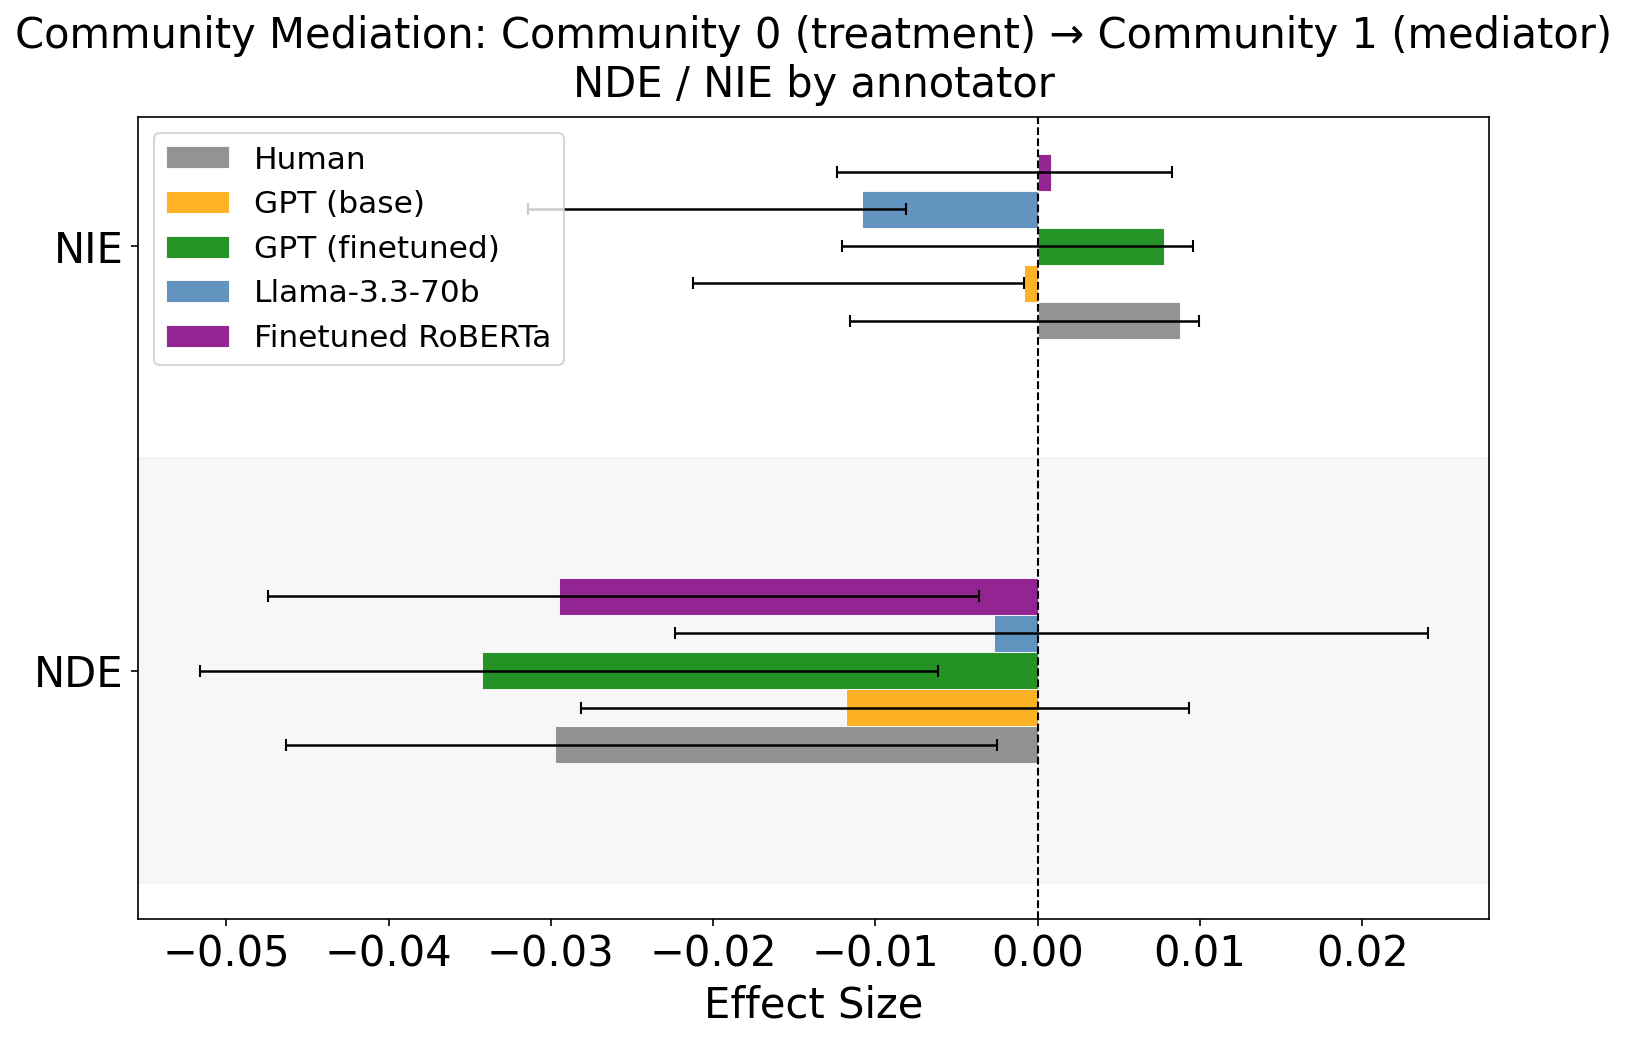
\includegraphics[width=\textwidth]{sections/images/causal_analysis/media_split/mediation_community_0_1.png}
        \caption{$0 \to 1$}
        \label{fig:mediation_0_1}
    \end{subfigure}
    \hfill
    \begin{subfigure}[b]{0.48\textwidth}
        \centering
        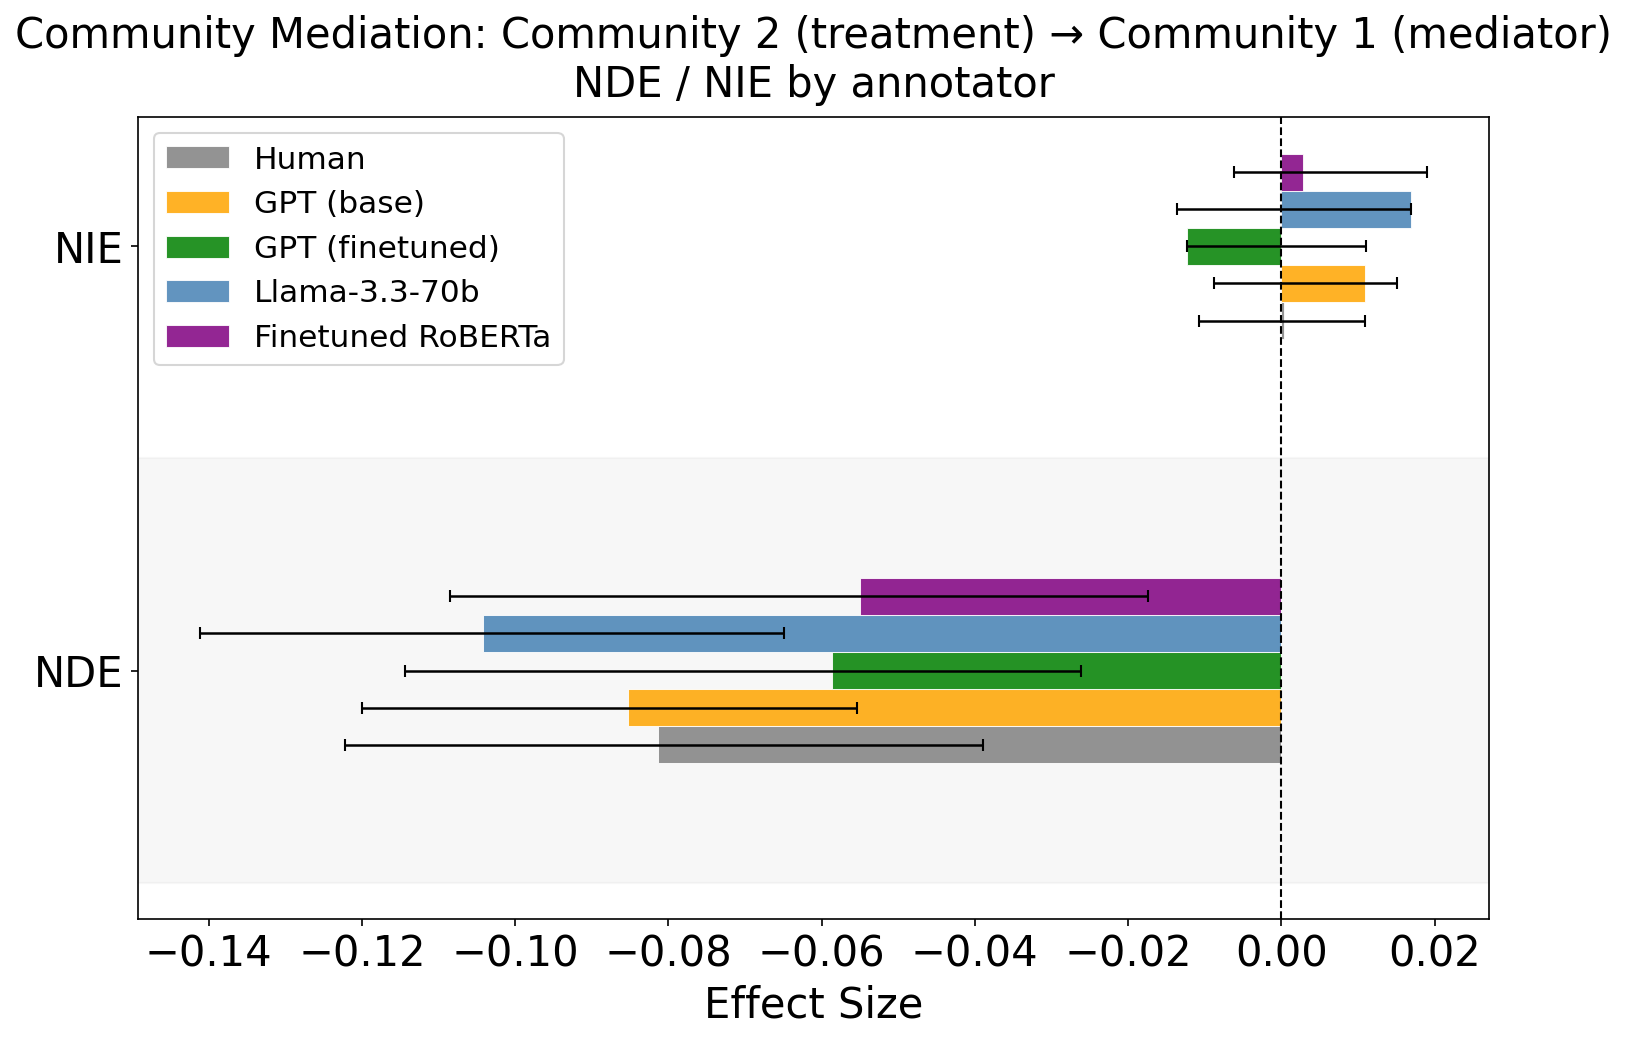
\includegraphics[width=\textwidth]{sections/images/causal_analysis/media_split/mediation_community_2_1.png}
        \caption{$2 \to 1$}
        \label{fig:mediation_2_1}
    \end{subfigure}
    \caption{Mediation decomposition with Community~1 (Elections and Campaigns) as mediator and Communities~0 (White House and Congress) and~2 (Public Health) as treatments. Serves as a contrast to Figure~\ref{fig:mediation_community_1_treatment}.}
    \label{fig:mediation_community_1_mediator}
\end{figure}

Across all four pathways, significance concentrates in the Natural Direct Effect rather than the Natural Indirect Effect. The implication is that sentiment toward one community shifts ideology predictions through a channel that does not flow through another community's sentiment; the mediating community carries little of the causal load.

The $1 \to 2$ pathway is the only configuration in which the estimated NIE changes direction across paradigms: Human ($+0.0045$), Fine-tuned RoBERTa ($+0.0069$), baseline GPT ($+0.0016$), and Fine-tuned GPT ($+0.0050$) all estimate a small positive indirect effect, while Llama-3.3-70B produces a small negative estimate ($-0.0001$). None of these NIEs reaches significance, so the reversal should not be over-interpreted, but it is worth noting that it occurs precisely where Community~2 (Public Health) acts as the mediator. Because Public Health is the community with full cross-paradigm ATE significance (Section~\ref{sec:community-level-results}), it is the strongest candidate for a genuine mediating channel, yet Llama alone routes its indirect effect in the opposite direction. This pattern warrants further investigation.

The confidence intervals are wide across all four pathways, typically spanning intervals of $0.15$ or more at the $Q_{25} \to Q_{75}$ contrast. Two factors plausibly contribute. First, sample sizes per pathway are modest: $1{,}116$ articles for the $2 \to 1$ pathway and $2{,}743$ articles for $0 \to 1$. Second, we use a simplified sentiment encoding: every annotation paradigm receives the same per-article community sentiment vectors, which likely does not capture all the nuance in how different paradigms interpret sentiment. A third consideration is the community-forming mechanism itself. Each community aggregates a large number of topics with heterogeneous political valences: Community~1 alone contains seven of the top~20 topics, including both right-coded (Donald Trump, Republican Party) and left-coded (Joe Biden, Hillary Clinton, Democratic Party) entities whose topic-level ATEs point in opposite directions. Aggregating sentiment over such a heterogeneous set partially cancels the underlying topic-level causal signals, which may explain why the community-level pathways show significance in the direct channel but rarely in the indirect channel is folded in. Smaller or more ideologically homogeneous communities might yield sharper decompositions.
